\documentclass{article}
\usepackage[utf8]{inputenc}
\usepackage[T1]{fontenc}
\usepackage{graphicx}
\usepackage{hyperref}
\usepackage{geometry}
\geometry{margin=1in}

\title{AMHURIST (Nicola}
\date{Encyclopaedia Britannica (1771)}

\begin{document}
\maketitle

\section*{Historical source}
\textbf{Entry ID:} \texttt{entry-amhurist-nicola-560} \\
\textbf{Volume ID:} 191253801 \\
\textbf{Character Count:} 979

\subsection*{Extracted Text}
AMHURIST (Nicola); an English poet and political writer, was born at Marden in Kent and entered of St. John's colleg, Oxford, I’d from whence he we accepted for irregularity of conduct and liberties principles. Retaining great recruitment against the answerfly on this occasion, the studied is a learning and discipline and forms of the molt etipecialable characters in it, in a poem published in 1742 called \_Coluba Britainans\_, and in a book entitled \_Terre Filosa\_. He published, a Nicechy on Poems, farred and profane ; and, The Convocation, a poem in five cantons, which was a false on the Billings of Rangers a magnonite. But he is left known for the flare he had in the political paper called \_Zie Grafjnaar\_ strongly, after having been the druge of his party for near 20 years, he was as much forge in the famous compromite of 1742 as if he had never been born ; and, when he died in that year of a broken hearts, was indented to the charity of the bookstler for a grave.



\section*{Source record}
\begin{itemize}
\item \textbf{Dataset:} \texttt{NationalLibraryOfScotland/encyclopaedia\_britannica\_illustrated}
\item \textbf{Dataset Revision:} \texttt{309f765b1ecc83e0a7f7762e44b4a927a7555443}
\item \textbf{Page ID:} \texttt{britannica:309f765b1ecc83e0a7f7762e44b4a927a7555443:train:560} \\
  \textbf{Filename:} \texttt{page-0560-c458f594fc79.jpg} \\
  \textbf{Row Index:} 560 \\
  \textbf{SHA256:} \texttt{c458f594fc79392e...}
\end{itemize}

\begin{figure}[h]
\centering
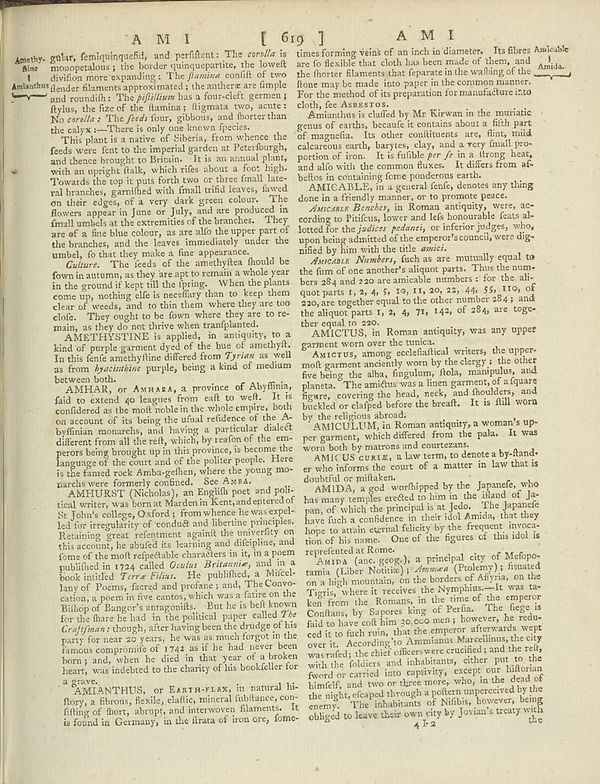
\includegraphics[width=0.85\textwidth]{../scans/page-0560-c458f594fc79.jpg}
\caption*{Source scan: \texttt{page-0560-c458f594fc79.jpg}}
\end{figure}

\end{document}
